\textbf{{1.电子邮件格式}}

1)电子邮件{\textbf{由信封和内容}}两部分组成。一般只规定了邮件内容中的首部格式,而邮件的主体部分由用户自由撰写。用户写好首部后,邮件系统自动将信封所需的信息提取出来并写在信封上。\\

2)邮件内容首部包含一些关键字,后面加上冒号,如``To:''是收信人的邮件地址、``Subject:''是邮件的主题等。

3)电子邮件地址的格式:收件人邮箱名@邮箱所在主机的域名,符号``@''读作``at'',表示``在''的意思。例如,电子邮件地址zhouwei@koudaitiku.com。

\textbf{{2.MIME}}

由于\textbf{SMTP}只限于传送一定长度的7位ASCII码邮件,于是提出了通用因特网邮件扩充(Multipurpose
Internet Mail Extensions,MIME)。MIME的意图是继续使用目前的{[}RFC
822{]}格式,但增加了邮件主体的结构,并定义了传送非ASCII码的编码规则。MIME与SMTP的关系如下图所示。

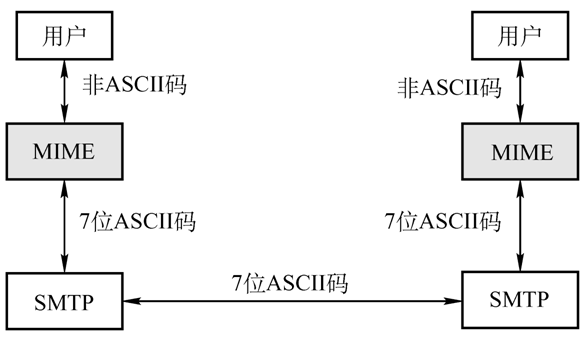
\includegraphics[width=3.43750in,height=1.96875in]{png-jpeg-pics/2E26762CC2097F8BF63CFE77B865092C.png}
